\documentclass[conference]{IEEEtran}

\usepackage[T1]{fontenc}
\usepackage[utf8]{inputenc}
\usepackage{amsmath,amssymb}
\usepackage{mathtools}
\usepackage[binary-units=true]{siunitx}
\DeclareSIUnit\eV{\electronvolt}
\DeclareSIUnit\amu{u}
\usepackage{booktabs}
\usepackage{graphicx}
\usepackage{tikz}
\usetikzlibrary{arrows.meta,positioning}
\usepackage[hidelinks]{hyperref}
\usepackage{xurl}
\usepackage[backend=biber,style=numeric-comp,sorting=none,giveninits=true,maxbibnames=6,minbibnames=3]{biblatex}
\setcounter{biburllcpenalty}{7000}
\setcounter{biburlucpenalty}{8000}
\addbibresource{refs/references_part1.bib}
\addbibresource{refs/references_part2.bib}
\addbibresource{refs/references_part3.bib}
\addbibresource{refs/references_part4.bib}

\newcommand{\Te}{T_{\mathrm{e}}}
\newcommand{\GammaE}{\Gamma_{E}}

\begin{document}

\title{Quantifying Ion Energy Flux Across Plasma Sheaths:\\ A Non-Intrusive, Physics-Constrained Optical Diagnostic Framework}

\author{
\IEEEauthorblockN{Nithisha V, Ajayaditya L, Denistan B}
\IEEEauthorblockA{\textit{Team Astrophage} \\
\textit{AIC RRCAT $\pi$-Hub Foundation, Department of Atomic Energy}\\
DIA Techathon 2.0 (Naari Shakti) --- Plasma Technologies for Industry \& Society}
}

\maketitle

\begin{abstract}
Ion energy flux across the plasma sheath governs the surface heating, erosion, and efficiency loss that limit the lifetime and performance of plasma-facing hardware in electric propulsion, semiconductor plasma etching, and fusion devices. First-principles models predict this flux, but it remains weakly validated because the available measurement tools fall short: intrusive electrostatic probes perturb the sheath they sample, while individual non-invasive optical diagnostics capture only a partial, usually time-averaged, slice of the plasma state. We propose a non-intrusive diagnostic framework that reconstructs ion energy flux by posing it as a physics-constrained inverse problem. Four mature, complementary optical diagnostics---optical emission spectroscopy, laser-induced fluorescence, Thomson scattering, and interferometry---are fused to over-determine the plasma state without inserting any object into the plasma, and the reconstruction is regularized with sheath theory and kinetic simulation. The result is a stable, spatially and temporally resolved estimate of the energy deposited at the wall. This paper states the measurement gap, formulates the framework and its forward and inverse structure, argues its feasibility through a staged validation plan, and outlines the application domains and commercialization pathway.
\end{abstract}

\begin{IEEEkeywords}
plasma sheath, ion energy flux, non-intrusive diagnostics, laser-induced fluorescence, Thomson scattering, inverse problems, physics-constrained inversion, electric propulsion, plasma etching, fusion.
\end{IEEEkeywords}

\section{Introduction}
At every boundary where a plasma meets a solid surface, ions accelerate across a thin, non-neutral layer---the sheath---and strike the wall. The energy they deposit per unit area per unit time, the ion energy flux $\GammaE$, sets three outcomes that make or break plasma technology: localized surface heating that caps the sustainable power density, sputter erosion that is the dominant wear mechanism and lifetime limiter, and the efficiency loss represented by energy delivered to walls rather than to thrust, etch precision, or confinement \cite{ref0001,ref0074}. The electrostatic structure of the plasma--wall transition and the Bohm criterion that fixes the ion flux entering the sheath are well established from fluid and kinetic theory \cite{ref0001,ref0166,ref0659}, and the consequences for erosion and heat loading are extensively documented \cite{ref0134,ref0562}.

Despite this predictive foundation, ion energy flux is not directly measurable, and its predictions remain weakly validated under realistic, non-equilibrium, and time-varying conditions. This paper argues that the gap is fundamentally a \emph{measurement} gap, and that closing it requires fusing several non-perturbing optical diagnostics under the constraint of first-principles sheath physics rather than improving any single instrument in isolation.

\section{The Measurement Gap}
Two families of diagnostic dominate current practice, and each is insufficient for validated ion-energy-flux measurement.

\emph{Intrusive probes.} Langmuir and related electrostatic probes yield electron temperature, density, and plasma potential from a current--voltage characteristic, but the inserted electrode forms its own sheath and perturbs the very structure under study; interpretation is further complicated in non-Maxwellian and magnetized regimes, and probes erode in high-flux environments \cite{ref0194,ref0195}. Retarding-field and emissive variants measure ion energy distributions but share the perturbation and survivability limitations \cite{ref0107}.

\emph{Single non-invasive optics.} Passive and laser-based optical methods are non-perturbing but each captures only a partial slice of the plasma state, and measurements are rarely time-resolved, so the transient sheath dynamics that drive erosion are averaged away. No single optical observable determines $\GammaE$, which is a functional of the ion velocity distribution function at the wall and therefore requires simultaneous constraints on density, temperature, and ion kinetics \cite{ref0074,ref0075}.

The consequence is the absence of a widely accepted, experimentally validated framework for quantifying ion energy transfer at plasma--surface boundaries.

\section{Proposed Framework}
We treat ion energy flux as an inverse problem: measure what optics can see without disturbing the plasma, constrain the reconstruction with first-principles physics, and solve for the quantity actually required (Fig.~\ref{fig:pipeline}).

\begin{figure}[t]
\centering
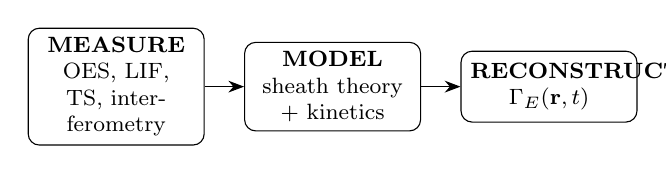
\begin{tikzpicture}[
  node distance=4mm and 5mm,
  box/.style={draw, rounded corners, align=center, font=\footnotesize,
              minimum height=9mm, text width=20mm},
  >={Stealth[length=2mm]}]
\node[box] (m) {\textbf{MEASURE}\\OES, LIF,\\TS, interferometry};
\node[box, right=of m] (p) {\textbf{MODEL}\\sheath theory\\+ kinetics};
\node[box, right=of p] (r) {\textbf{RECONSTRUCT}\\$\GammaE(\mathbf{r},t)$};
\draw[->] (m) -- (p);
\draw[->] (p) -- (r);
\end{tikzpicture}
\caption{Schematic (illustrative) of the physics-constrained inversion pipeline: non-perturbing optical observables are combined with first-principles priors to reconstruct the spatially and temporally resolved ion energy flux.}
\label{fig:pipeline}
\end{figure}

\subsection{Four Complementary Non-Perturbing Diagnostics}
Each technique is individually mature; together they over-determine the plasma state, which is the redundancy that makes the reconstruction well posed.
\begin{itemize}
\item \textbf{Optical emission spectroscopy (OES)} infers electron temperature and excited-species densities from the plasma's own emission via line-ratio and collisional--radiative analysis, with zero perturbation \cite{ref0227,ref0260,ref0261}.
\item \textbf{Laser-induced fluorescence (LIF)} reconstructs the ion velocity distribution function through Doppler-resolved excitation---the most direct optical access to ion energetics at the boundary \cite{ref0292,ref0328,ref0329}.
\item \textbf{Thomson scattering (TS)} provides a direct, spatially local, model-light measurement of electron temperature and density \cite{ref0354,ref0355}.
\item \textbf{Interferometry} yields a fast, robust line-integrated electron density from optical phase shift \cite{ref0388,ref0389}.
\end{itemize}
Table~\ref{tab:diag} summarizes the observables and their role in the fusion.

\begin{table}[t]
\caption{Complementary diagnostics fused in the framework.}
\label{tab:diag}
\centering
\footnotesize
\begin{tabular}{@{}lll@{}}
\toprule
\textbf{Technique} & \textbf{Primary observable} & \textbf{Perturbs?} \\
\midrule
OES & $\Te$, excited-species densities & no \\
LIF & ion velocity distribution & no \\
Thomson scattering & $\Te$, $n_{\mathrm{e}}$ (local) & no \\
Interferometry & $n_{\mathrm{e}}$ (line-integrated) & no \\
Langmuir probe & $\Te$, $n_{\mathrm{e}}$, $V_{\mathrm{p}}$ & \textbf{yes} \\
\bottomrule
\end{tabular}
\end{table}

\subsection{Physics-Constrained Inversion}
Let $\mathbf{m}$ denote the unknown bulk, presheath, and sheath state (densities, temperatures, an ion-velocity-distribution basis, and sheath-structure parameters), and let $\mathbf{d}$ be the concatenated calibrated outputs of the four diagnostics. The forward model $\mathbf{G}$ maps state to observables,
\begin{equation}
\mathbf{d} = \mathbf{G}(\mathbf{m}) + \boldsymbol{\varepsilon}, \qquad \boldsymbol{\varepsilon}\sim\mathcal{N}(\mathbf{0},\boldsymbol{\Sigma}),
\end{equation}
and the target is the nonlinear functional
\begin{equation}
\GammaE = \tfrac{1}{2} m_{\mathrm{i}} \int_{0}^{\infty} v^{3}\, f_{\mathrm{i}}^{\mathrm{wall}}(v)\,\mathrm{d}v .
\end{equation}
Because $\GammaE$ is not directly observable and any single channel is rank-deficient, the reconstruction is posed as a regularized estimation problem,
\begin{equation}
\hat{\mathbf{m}} = \arg\min_{\mathbf{m}}\ \big\lVert \mathbf{G}(\mathbf{m})-\mathbf{d}\big\rVert_{\boldsymbol{\Sigma}^{-1}}^{2} + \alpha\, \mathcal{R}(\mathbf{m}),
\end{equation}
where the regularizer $\mathcal{R}$ encodes sheath theory and kinetic-simulation priors. This is the same estimation philosophy as integrated data analysis in fusion \cite{ref0706,ref0707}, specialized to the sheath boundary layer, and it draws on established regularized-inversion practice in plasma spectroscopy and tomography \cite{ref0677,ref0678}. Kinetic and particle-in-cell models supply both the forward operator and synthetic ground truth for validation \cite{ref0631,ref0632,ref0660}.

\subsection{Time-Resolved by Design}
Sheaths are non-equilibrium and, in radio-frequency sources, strongly time-dependent, producing bimodal ion energy distributions \cite{ref0038,ref0039}. Time-resolved acquisition captures the transient energy spikes that steady-state methods average away, which is essential for accurate erosion prediction \cite{ref0135}.

\section{Feasibility and Validation}
The framework is de-risked by a staged plan in which each stage produces a checkable result before the next. First, analytical sheath models and kinetic simulations are used to build and validate the inversion on synthetic data, recovering a known flux from simulated observables. Second, OES, LIF, and interferometry are stood up on a controlled plasma source and the reconstruction is tested against measurements. Third, Thomson scattering is added with advanced laser and vacuum infrastructure for high-resolution validation under realistic conditions. Every diagnostic is individually proven \cite{ref0261,ref0355,ref0389}; the novelty is the fusion and inversion, not the hardware. The principal assumptions still under validation are the well-posedness of the inversion under measurement noise, optical-access geometry on target hardware, and cross-diagnostic calibration.

\section{Application Domains}
\subsection{Electric and Space Propulsion}
Hall and gridded ion thrusters accelerate ions to produce efficient thrust, but the same ions erode channel walls and grids; erosion is the dominant life-limiting mechanism and the central obstacle to qualification \cite{ref0424,ref0425,ref0459,ref0460,ref0489,ref0490}. A non-intrusive $\GammaE$ diagnostic enables lifetime prediction and design optimization without disturbing operation.

\subsection{Semiconductor Plasma Etching}
In reactive ion etching the sheath accelerates ions into the wafer, and the ion energy and angular distribution set anisotropy, selectivity, and damage; at advanced nodes this control is decisive for yield \cite{ref0513,ref0514,ref0539,ref0540}. In-situ ion-energy-flux measurement tightens process control.

\subsection{Fusion Plasma-Facing Components}
The divertor and first wall endure extreme heat and particle loads, and plasma-facing erosion and heat handling remain top unsolved barriers to viable fusion \cite{ref0562,ref0563,ref0594,ref0595}. A validated non-intrusive flux diagnostic addresses this pain point directly.

\section{Roadmap and Commercialization}
The framework is positioned not as competing hardware but as the measurement and qualification layer that propulsion developers, semiconductor fabs, and fusion laboratories depend on. The product is a non-intrusive diagnostic package---optical hardware bundled with the physics-constrained inversion software---monetized as diagnostic systems, inversion-software licensing, and qualification-as-a-service. The near-term path is incubation within the DIA ecosystem, access to advanced laser and vacuum infrastructure, a partner pilot for field qualification, and productization.

\section{Conclusion}
Ion energy flux decides how plasma hardware heats, erodes, and lasts, yet today it cannot be measured without disturbing the plasma. By fusing four non-perturbing optical diagnostics with first-principles sheath physics and solving a regularized inverse problem, the proposed framework reconstructs this flux in a validated, spatially and temporally resolved way. It becomes a diagnostics-and-qualification layer serving electric propulsion, semiconductor etching, and fusion---three large and growing plasma-driven markets united by the same plasma--surface boundary.

\section*{Acknowledgment}
The authors thank the AIC RRCAT $\pi$-Hub Foundation, RRCAT and the Department of Atomic Energy, the DAE Incubator Alliance, and the Atal Innovation Mission (NITI Aayog) for the DIA Techathon 2.0 platform.

\printbibliography

\end{document}
